\documentclass[12pt]{article}
\usepackage{amsmath}
\usepackage{tikz}
\usepackage{qtree}
\usepackage{mathtools}
\usetikzlibrary{automata, positioning, arrows}

\tikzset{node distance=2.5cm,
	every state/.style={semithick, fill=gray!10},
	initial text={},
	double distance=2pt,
	every edge/.style={draw, ->, >=stealth, auto, semithick}}

%\tikzset{->,
%	>=stealth,
%	node distance=3cm,
%	every state/.style={thick, fill=gray!10}, initial text=$ $,}

\title{CENG280 Homework 2}
\author{Murat Bolu}
\date{2521300}

\begin{document}

\maketitle

\section*{Answer 1}

\begin{center}
    Let $G_1$ be the quadruple $(V, \Sigma, R, S)$ where
\end{center}
\begin{align*}
    V = \{&a, b, S\}, \\
    \Sigma = \{&a, b\}, \\
    R = \{&S \rightarrow e \mid SS \\
    &\hspace{32 pt} \mid abbS \mid abSb \mid aSbb \mid Sabb \\
    &\hspace{32 pt} \mid babS \mid baSb \mid bSab \mid Sbab \\
    &\hspace{32 pt} \mid bbaS \mid bbSa \mid bSba \mid Sbba\} \\
\end{align*}

\section*{Answer 2}

\begin{center}
    Let $G_2$ be the quadruple $(V, \Sigma, R, S)$ where
\end{center}
\begin{align*}
    V = \{&a, b, S\}, \\
    \Sigma = \{&a, b\}, \\
    R = \{&S \rightarrow e \mid aSb \mid aaSb\} \\
\end{align*}

\newpage

\section*{Answer 3}

\begin{center}
    Let $M_1$ be the sextuple $(K, \Sigma, \Gamma, \Delta, s, F)$ where
\end{center}
\begin{align*}
    K = \{&s, f\} \\
    \Sigma = \{&a, b\} \\
    \Gamma = \{&a, b, S\} \\
    F = \{&f\} \\
    \Delta = \{&((s, e, e),(f, S)), \\
    &((f, e, S),(f, e)), ((f, e, S),(f, SS)), \\
    &((f, e, S),(f, abbS)), ((f, e, S),(f, abSb)), \\
    &((f, e, S),(f, aSbb)), ((f, e, S),(f, Sabb)), \\
    &((f, e, S),(f, babS)), ((f, e, S),(f, baSb)), \\
    &((f, e, S),(f, bSab)), ((f, e, S),(f, Sbab)), \\
    &((f, e, S),(f, bbaS)), ((f, e, S),(f, bbSa)), \\
    &((f, e, S),(f, bSba)), ((f, e, S),(f, Sbba)), \\
    &((f, a, a),(f, e)), ((f, b, b),(f, e))\} \\
\end{align*}

\begin{figure}[ht]
\centering
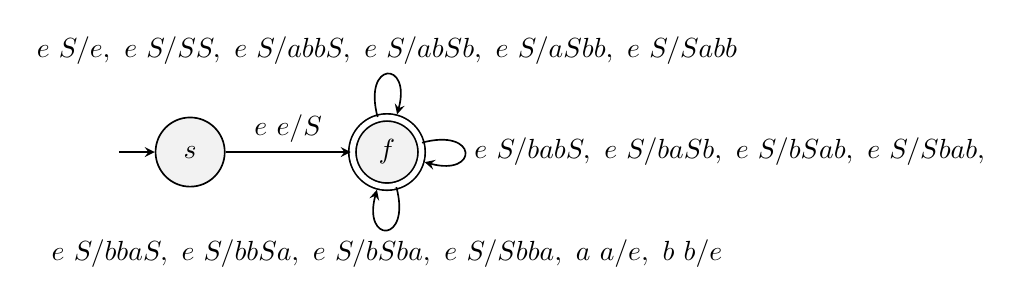
\begin{tikzpicture}
    \node[state, initial] (s) {$s$};
    \node[state, accepting, right of=s] (f) {$f$};
    \draw (s) edge[above] node{$e\ e/S$} (f);
    \draw (f) edge[loop above] node{$e\ S/e,\ e\ S/SS,\ e\ S/abbS,\ e\ S/abSb,\ e\ S/aSbb,\ e\ S/Sabb$} (f);
    \draw (f) edge[loop right] node{$e\ S/babS,\ e\ S/baSb,\ e\ S/bSab,\ e\ S/Sbab,$} (f);
    \draw (f) edge[loop below] node{$e\ S/bbaS,\ e\ S/bbSa,\ e\ S/bSba,\ e\ S/Sbba,\ a\ a/e,\ b\ b/e$} (f);
\end{tikzpicture}
\end{figure}

\newpage

\section*{Answer 4}

\begin{center}
    Let $G_3$ be the quadruple $(V, \Sigma, R, S)$ where
\end{center}
\begin{align*}
    V = \{&a, b, S\}, \\
    \Sigma = \{&a, b\}, \\
    R = \{&S \hspace{4 pt} \rightarrow S_1 \mid S_2, \\
    &S_1 \rightarrow \hspace{6.5 pt} e \mid S_1S_1 \\
    &\hspace{42.5 pt} \mid abbS_1 \mid abS_1b \mid aS_1bb \mid S_1abb \\
    &\hspace{42.5 pt} \mid babS_1 \mid baS_1b \mid bS_1ab \mid S_1bab \\
    &\hspace{42.5 pt} \mid bbaS_1 \mid bbS_1a \mid bS_1ba \mid S_1bba, \\
    &S_2 \rightarrow \hspace{6.5 pt} e \mid aS_2b \mid aS_2bb\}
\end{align*}

\section*{Answer 5}

\begin{center}
The string $00111$ can be parsed in two different ways, showing that $G_1$ is ambigiuous.
\end{center}

\Tree[.$S$
         [.$A$
             [.$A$
                 [.$0$
                 ]
                 [.$A$
                     [.$0$
                     ]
                     [.$1$
                     ]
                 ]
                 [.$1$
                 ]
             ]
             [.$1$
             ]
         ]
         [.$S$
             [$e$
             ]
         ]
     ]

\Tree[.$S$
         [.$A$
             [.$0$
             ]
             [.$A$
                 [.$A$
                     [.$0$
                     ]
                     [.$1$
                     ]
                 ]
                 [.$1$
                 ]
             ]
             [.$1$
             ]
         ]
         [.$S$
             [$e$
             ]
         ]
     ]

\newpage

\section*{Answer 6}

\begin{center}
    Let $G_b$ be the quadruple $(V, \Sigma, R, S)$ where
\end{center}
\begin{align*}
    V = \{&0, 1, S, A, B\}, \\
    \Sigma = \{&0, 1\}, \\
    R = \{&S \rightarrow AS \mid e, \\
    &A \rightarrow 0A1 \mid 0B, \\
    &B \rightarrow B1 \mid 1\}
\end{align*}

\section*{Answer 7}

\begin{align*}
S &\xRightarrow{L} AS \\
&\xRightarrow{L} 0A1S \\
&\xRightarrow{L} 00B1S \\
&\xRightarrow{L} 00B11S \\
&\xRightarrow{L} 00111S \\
&\xRightarrow{L} 00111 \\
\end{align*}

\Tree[.$S$
         [.$A$
             [.$0$
             ]
             [.$A$
                 [.$0$
                 ]
                 [.$B$
                     [.$B$
                         [.$1$
                         ]
                     ]
                     [.$1$
                     ]
                 ]
             ]
             [.$1$
             ]
         ]
         [.$S$
             [$e$
             ]
         ]
     ]

\end{document}
